\documentclass[english]{panikzettel}

\usepackage{nccmath}
\usepackage{graphicx}
\usepackage[nameinlink]{cleveref}

\usetikzlibrary{arrows,intersections,automata,matrix,calc}
\renewcommand\deg{\textsf{deg}}
\newcommand{\N}{\mathbb{N}}
\renewcommand\O{\mathcal{O}}
\newcommand{\R}{\mathbb{R}}

\tikzset{
    vertex/.style = {circle,
                    fill=white,
                    draw=black,
                    text=black,
                    very thick,
                    inner sep=2pt},
    pebble/.style = {circle,
                    fill=none,
                    draw=black,
                    dashed,
                    text=black,
                    ultra thick,
                    inner sep=4pt},
    box/.style = 	{rectangle,
                    rounded corners,
                    fill=white!90!black,
                    draw=black,
                    text=black,
                    ultra thick,
                    inner sep=12pt},
    -,
    node/.style =   {circle,
                    fill=white,
                    draw=dg,
                    text=black,
                    very thick,
                    minimum width={width("MMMMM")+1pt}},
    S/.style =      {rectangle,
                    fill=white,
                    draw=dg,
                    text=black,
                    very thick,
                    minimum width={width("MM")+1pt}},
    P/.style    =   {circle,
                    fill=white,
                    draw=dg,
                    text=black,
                    very thick,
                    minimum width={width("MM")+1pt}},
    -,
    every to={draw,dashed},
    >=stealth',
    shorten >= 1pt,
    shorten <= 1pt,
    node distance=2cm,
    draw=white!20!black}

\title{Social Networks\textsuperscript{2019} Panikzettel}
\author{Luca Oeljeklaus, Caspar Zecha, Philipp Schröer}

\begin{document}

\maketitle

\tableofcontents

\section*{Introduction}

This Panikzettel covers the lecture Social Networks, held in the summer semesters of 2019 and 2020 by Prof.~Dr.~Markus Strohmaier.

\definecolor{panikgreen}{HTML}{2AA198}
\begin{tcolorbox}[
    colframe=panikgreen,
    colback=white,
    toprule=0pt,
    boxrule=0.75pt,
]
    \sffamily
    We have two Panikzettel on Social Networks!
    This one was mainly written in the summer semester of 2019.
    Daniel Sous also wrote one in 2020: \href{https://panikzettel.philworld.de/sn20.pdf}{Social Networks 2020 Panikzettel}.
\end{tcolorbox}

This Panikzettel is Open Source. We appreciate comments and suggestions at \\
\url{https://git.rwth-aachen.de/philipp.schroer/panikzettel}.

\section{Graphs}

A \textit{simple graph} is a tuple $G = \big(V(G),E(G)\big)$, where $V(G)$ is a finite set of \textit{vertices} (or \textit{nodes}) and $E(G) \subseteq \mbinom{V(G)}{2}$ is a set of \textit{edges} (or \textit{links}).

An \textit{undirected graph} $G$ satisfies for all $v,w \in V(G)$ that $(v,w) \in E(G) \Leftrightarrow (w,v) \in E(G)$.
We also just write $vw \in E(G)$ instead of $(v,w) \in E(G)$ for undirected $G$.

A \textit{directed graph} (or \textit{digraph}) is a graph which is not undirected.

A \textit{weigthed graph} $G$ has a weight function $w: V(G) \to W$ (where $W$ is usually $\mathbb{Q}$ or $\mathbb{R}$) to every edge.
A graph which does not is called \textit{binary} (either an edge exists or it does not).

A \textit{simple multigraph} is a graph where $E(G)$ is a multiset (there may be several edges with the same source and target).
It may also contain self-loops: there may exist $v\in V(G)$ such that $vv \in E(G)$.

A digraph $G$ contains a cycle if there exists a set of edges $v_1v_2,\dots,v_{n-1}v_n,v_nv_1 \in E(G)$ for an $n \ge 2$. A digraph is \textit{acyclic} if it does not contain a cycle.

Given some graph $G$, we generally refer to the number of vertices by $n$ and to the number of edges by $m$.

We denote by $N_G(v) = \Set{w|vw \in E(G)}$ the \textit{neighbourhood} of $v$ in $G$.
We may omit the subscript if it is clear from context.
Similarly, we denote by $N_G(v,w) = \Set{y|vy \in E(G) \lor wy \in E(G)}$ the set of common neighbours of $v$ and $w$.

We refer to the average degree of a graph as $\langle k \rangle$.
For a vertex $v$, the degree of $v$ may be written as $\deg_G(v)$, $k_v$ or $|N_G(v)|$.
When talking about in- or out-degrees, we generally add an $^{in}$ or $^{out}$ superscript.

\subsection{Adjacency Matrix}

Let $G = (V(G),E(G))$ be a digraph.
The \textit{adjacency matrix} $A \in \Set{0,1}^{n\times n}$ of $G$ is given by:
\[
    A_{ij} = \begin{cases}
        1, \text{ if } ij \in E(G), \\
        0, \text{ otherwise.}
    \end{cases}
\]

When considering weighted graphs, we let $A_{ij} = w_{ij}$.

The \textit{density} of an undirected graph is given by $\frac{|E(G)|}{\left|\mbinom{V(G)}{2}\right|} = \frac{2\cdot |E(G)|}{|V(G)| \cdot (|V(G)| -1) }$.

We call a graph \emph{sparse} if $|E(G)| \approx |V(G)|$.
In these cases, an adjacency matrix is an inefficient way of storing the graph.
A graph for which the number of edges is significantly larger than the number of vertices is called \textit{dense}.
Most observed graphs are sparse.

An alternative representation for sparse graph is the \textit{edge list}, where we simply store a list of edges where every edge is represented by a 2-tuple containing its source and its target vertex (for weighted edges, we may use 3-tuples, where the third stored value is the weight of the edge).

\subsection{Clustering Coefficient}

For undirected graphs, the \textit{clustering coefficient} is a measure of how connected the neighbourhood of a vertex is.
For some $v \in V(G)$ it is given by $$c_v = \frac{2 \cdot e_v}{\deg_G(v)\cdot(\deg_G(v)-1)},$$
where $e_v$ is the number of edges between the neighbours of $v$.
The clustering coefficient of a graph is given by: $$C_G = \frac{1}{|V(G)|} \cdot \sum_{v \in V(G)} c_v.$$

An alternative to the clustering coefficient is the \textit{potential triangle count}, which is given by: $$P_G = \frac{\text{number of triangles} \cdot 3}{\text{number of connected triples}}.$$

\subsection{Small World Property} \label{sec:small-world}

\begin{halfboxl}
    A graph $G$ satisfies the \textit{small world property} if it has, compared to a random graph $G'$ of the same order, more or less the same average path length $L_G$ and a much higher clustering coefficient.
\end{halfboxl}%
\begin{halfboxr}
    \vspace{-\baselineskip}
     \begin{defi}{Small World Property}
        Formally, $G$ must satisfy $\sigma = \frac{\frac{C_G}{C_{G'}}}{\frac{L_G}{L_{G'}}} > 1$.
    \end{defi}
\end{halfboxr}

\subsection{Components and Paths}

In a graph where more than $90\%$ of vertices are contained in a single component, we refer to that component as the \textit{giant component}.

A digraph is \textit{strongly connected} if for every pair of vertices there exists a path leading from one to the other and vice versa.
It is \textit{weakly connected} if this is satisfied for at least one direction.

Components can be identified with \emph{Depth First Search} (DFS) or \emph{Breadth First Search} (BFS).

\begin{halfboxl}
    \vspace{-\baselineskip}
    \begin{algo}{Depth First Search}
        \textbf{Input:} A graph $G$, a vertex $v$.\\
        \textbf{Output:} All nodes reachable from $v$.
        \tcblower
        \begin{enumerate}
            \item Label $v$ as discovered.
            \item For all neighbours $w$ of $v$:
            \begin{enumerate}
                \item If $w$ is not labeled as discovered:
                \begin{enumerate}
                    \item Recursively call $DFS$ with $G$ and $w$.
                \end{enumerate}
            \end{enumerate}
            \item Return discovered nodes.
        \end{enumerate}
    \end{algo}
\end{halfboxl}%
\begin{halfboxr}
    \vspace{-\baselineskip}
    \begin{algo}{Breadth First Search}
        \textbf{Input:} A graph $G$, a vertex $v$.\\
        \textbf{Output:} All nodes reachable from $v$.
        \tcblower
        \begin{enumerate}
            \item Label $v$ as discovered.
            \item Create queue $Q$ and enqueue $v$ onto $Q$.
            \item While $Q$ is not empty:
                \begin{enumerate}
                    \item Dequeue $w$ from $Q$:
                    \item For all neighbours $x$ of $w$ that are not labeled as discovered:
                        \begin{enumerate}
                            \item Label $x$ as discovered.
                            \item Enqueue $x$ onto $Q$.
                        \end{enumerate}
                \end{enumerate}
            \item Return discovered nodes.
        \end{enumerate}
    \end{algo}
\end{halfboxr}

\subsubsection*{Dijsktra's Algorithm}

\textit{Dijsktra's algorithm} is used to compute the shortest path (also called \emph{geodesic path}) from one vertex to all the others.
This version here stops when a certain destination node is discovered.

\begin{algo}{Dijsktra's Algorithm}
    \textbf{Input:} A graph $G$, an initial vertex $v$, a destination vertex $z$.\\
    \textbf{Output:} A distance function $d:V(G) \to \N$ which assigns every $w \in V(G)$ its distance to $v$.
    \tcblower
    \begin{enumerate}
        \item Create queue $Q$ of all vertices, and set distance $d(v) = 0$ and $d(w) = \infty$ for all other $w \in V(G)$. Label all nodes as undiscovered.
        \item While $Q$ is not empty:
            \begin{enumerate}
                \item Dequeue the node $w$ with smallest tentative distance $d(w)$ from $Q$ and label it as discovered.
                \item If $w$ is the destination node $z$ then terminate.
                \item For each neighbour $x$ of $w$ that has not been labeled as discovered:
                    \begin{enumerate}
                        \item Compute the tentative distance $d(x)$: The smallest value between the current distance $d(x)$ and the sum of the distance $d(w)$ plus the weight of the edge $(w,x)$.
                    \end{enumerate}
            \end{enumerate}
    \end{enumerate}
\end{algo}

The length of the longest shortest path of a graph is called the \emph{diameter} of the graph.

\subsection{Centrality Measures}

There are a few different graph metrics which are referred to as \textit{centrality measures}.
These centrality measures compute a score for every vertex which tells us how central it is to the network it is located in.

\begin{defi}{Degree Centrality}
    For a digraph, the \textit{degree centralities} of a vertex are given by:
    \[
        dc_v^{\text{in}} = \sum_{w\in V(G)} A_{vw} \quad\text{ and }\quad dc_v^{\text{out}} = \sum_{w\in V(G)} A_{wv}.
    \]

    For undirected (weighted) graphs it is given by: $dc_v = \sum_{w\in V(G)} A_{vw}$.

    The above centralities can be normalised by dividing by $n-1$.
\end{defi}

However, degree centrality is a local measure and does not take into account the location of a vertex in a network.

\begin{defi}{Closeness Centrality}
    The \textit{closeness centrality} of a vertex $v$ is given by: $$cc_v = \frac{1}{d_v},$$ where $d_v = \frac{1}{n-1} \sum_{w \neq v} d_{vw}$ is the average distance from $v$ to all other vertices.
    A high closeness centrality implies that a vertex is on average close to all other vertices.
\end{defi}

Closeness centrality is already more precise than degree centrality.
However, in small diameter networks it often turns out to be ineffective as the range of values is too narrow.
It is also very sensitive to variations in the network.
Further, it is undefined in networks with multiple components.

\begin{defi}{Betweenness Centrality}
    The \textit{betweenness centrality} of a vertex $v$ is given by: $$bc_i = \sum_{v,w\in V(G)} \frac{\textsf{sp}(v,i,w)}{\textsf{sp}(v,w)},$$ where $\textsf{sp}(v,w)$ is the number of shortest paths from $v$ to $w$, while $\textsf{sp}(v,i,w)$ is the number of shortest pathes from $v$ to $w$ that pass through $i$.
\end{defi}

Betweenness centrality, while pretty good, is limited to shortest paths, while generally information can travel long distances.
Furthermore, it has time complexity $\mathcal{O}(n^3)$, which is pretty bad.

\paragraph{Eigenvector Centrality}

\textit{Eigenvector centrality} is a measure of the influence of a node and is computed recursively.
Initially, every vertex $v$ is assigned $ec_v = 1$.
In every step, it is then updated by assigning each vector the sum of the centralities of the neighbours, normalised by the maximum observed centrality.

\paragraph{PageRank}

\textit{PageRank} works in a similar way to eigenvector centrality.
Every vertex is initialised to the value $\frac{1}{n}$ and in every turn, the value of every vertex is divided by its number of out-edges and sent to its neighbours until the values converge.

\begin{center}
    \begin{tabular}{cc}
        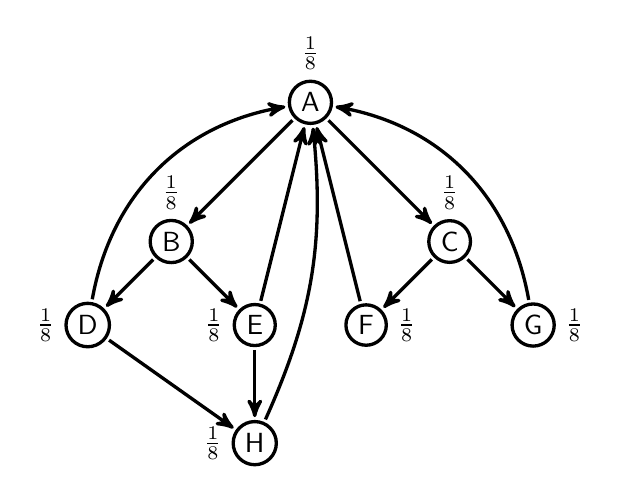
\begin{tikzpicture}[node distance=1.5cm]
                \node[vertex]       (A) [label={above:$\frac{1}{8}$}]                  					{\textsf{A}};
                \node[vertex]       (B) [below left of=A,node distance=2.5cm,label={above:$\frac{1}{8}$}]   {\textsf{B}};
                \node[vertex]       (C) [below right of=A,node distance=2.5cm,label={above:$\frac{1}{8}$}]  {\textsf{C}};
                \node[vertex]       (D) [below left of=B,label={left:$\frac{1}{8}$}]   					{\textsf{D}};
                \node[vertex]       (E) [below right of=B,label={left:$\frac{1}{8}$}]  					{\textsf{E}};
                \node[vertex]       (F) [below left of=C,label={right:$\frac{1}{8}$}]   					{\textsf{F}};
                \node[vertex]       (G) [below right of=C,label={right:$\frac{1}{8}$}]  					{\textsf{G}};
                \node[vertex]       (H) [below of=E,label={left:$\frac{1}{8}$}]  							{\textsf{H}};

                \path [very thick,->]  	(A) edge []             node [] {} (B)
                                        (A) edge []             node [] {} (C)
                                        (B) edge []             node [] {} (D)
                                        (B) edge []             node [] {} (E)
                                        (C) edge []             node [] {} (F)
                                        (C) edge []             node [] {} (G)
                                        (D) edge [bend left=35]             node [] {} (A)
                                        (D) edge []             node [] {} (H)
                                        (E) edge []             node [] {} (A)
                                        (E) edge []             node [] {} (H)
                                        (F) edge []             node [] {} (A)
                                        (G) edge [bend right=35]             node [] {} (A)
                                        (H) edge [bend right=15]             node [] {} (A);
        \end{tikzpicture} & 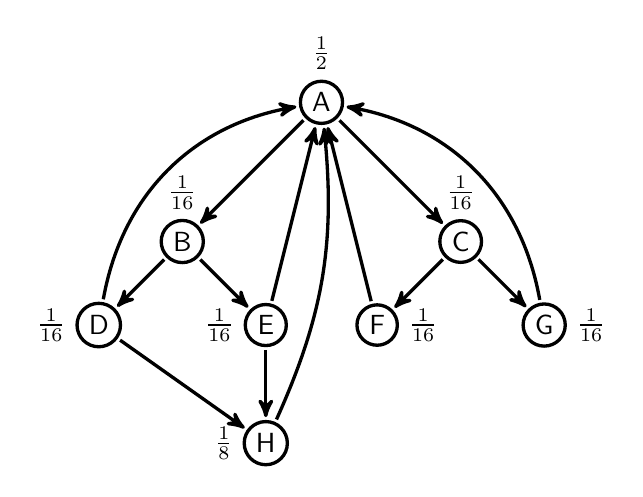
\begin{tikzpicture}[node distance=1.5cm]
                \node[vertex]       (A) [label={above:$\frac{1}{2}$}]                  					{\textsf{A}};
                \node[vertex]       (B) [below left of=A,node distance=2.5cm,label={above:$\frac{1}{16}$}]   {\textsf{B}};
                \node[vertex]       (C) [below right of=A,node distance=2.5cm,label={above:$\frac{1}{16}$}]  {\textsf{C}};
                \node[vertex]       (D) [below left of=B,label={left:$\frac{1}{16}$}]   					{\textsf{D}};
                \node[vertex]       (E) [below right of=B,label={left:$\frac{1}{16}$}]  					{\textsf{E}};
                \node[vertex]       (F) [below left of=C,label={right:$\frac{1}{16}$}]   					{\textsf{F}};
                \node[vertex]       (G) [below right of=C,label={right:$\frac{1}{16}$}]  					{\textsf{G}};
                \node[vertex]       (H) [below of=E,label={left:$\frac{1}{8}$}]  							{\textsf{H}};

                \path [very thick,->]  	(A) edge []             node [] {} (B)
                                        (A) edge []             node [] {} (C)
                                        (B) edge []             node [] {} (D)
                                        (B) edge []             node [] {} (E)
                                        (C) edge []             node [] {} (F)
                                        (C) edge []             node [] {} (G)
                                        (D) edge [bend left=35]             node [] {} (A)
                                        (D) edge []             node [] {} (H)
                                        (E) edge []             node [] {} (A)
                                        (E) edge []             node [] {} (H)
                                        (F) edge []             node [] {} (A)
                                        (G) edge [bend right=35]             node [] {} (A)
                                        (H) edge [bend right=15]             node [] {} (A);
        \end{tikzpicture} \\
        Initialisation & First Iteration \\
    \end{tabular}

    In this diagram: The first iteration of PageRank exemplified.
\end{center}


\paragraph{Scaled PageRank}

In some graphs, PageRank results in all the value being concentrated into few vertices which act as sinks.
To counteract this, after every step, \textit{scaled page rank} scales down the value of each vertex equally by some $s$ and redistributes the rest equally to all nodes such that the sum becomes one again.
Formally, this means that:
\[
    \textsf{PR}(i) = \frac{1-s}{n}+s \cdot \sum_{\forall j: i \in N_G(j)}\frac{\textsf{PR}(j)}{\deg^{out}_G(j)}.
\]

\begin{center}
    \begin{tabular}{cc}
        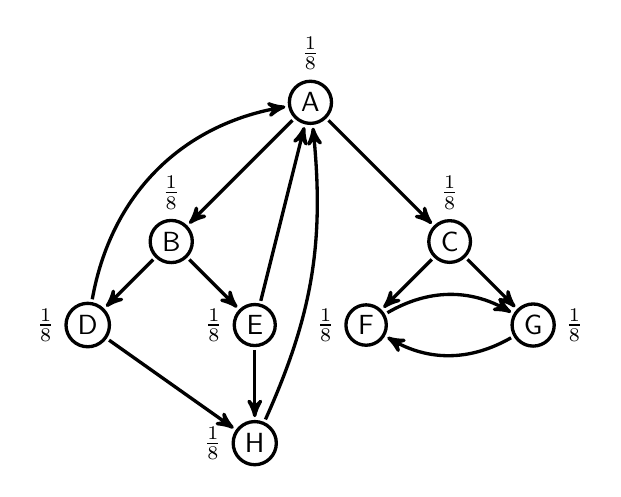
\begin{tikzpicture}[node distance=1.5cm]
                \node[vertex]       (A) [label={above:$\frac{1}{8}$}]                  						{\textsf{A}};
                \node[vertex]       (B) [below left of=A,node distance=2.5cm,label={above:$\frac{1}{8}$}]   {\textsf{B}};
                \node[vertex]       (C) [below right of=A,node distance=2.5cm,label={above:$\frac{1}{8}$}]  {\textsf{C}};
                \node[vertex]       (D) [below left of=B,label={left:$\frac{1}{8}$}]   						{\textsf{D}};
                \node[vertex]       (E) [below right of=B,label={left:$\frac{1}{8}$}]  						{\textsf{E}};
                \node[vertex]       (F) [below left of=C,label={left:$\frac{1}{8}$}]   					{\textsf{F}};
                \node[vertex]       (G) [below right of=C,label={right:$\frac{1}{8}$}]  					{\textsf{G}};
                \node[vertex]       (H) [below of=E,label={left:$\frac{1}{8}$}]  							{\textsf{H}};

                \path [very thick,->]  	(A) edge []             node [] {} (B)
                                        (A) edge []             node [] {} (C)
                                        (B) edge []             node [] {} (D)
                                        (B) edge []             node [] {} (E)
                                        (C) edge []             node [] {} (F)
                                        (C) edge []             node [] {} (G)
                                        (D) edge [bend left=35]             node [] {} (A)
                                        (D) edge []             node [] {} (H)
                                        (E) edge []             node [] {} (A)
                                        (E) edge []             node [] {} (H)
                                        (F) edge [bend left]             node [] {} (G)
                                        (G) edge [bend left]             node [] {} (F)
                                        (H) edge [bend right=15]             node [] {} (A);
        \end{tikzpicture} & 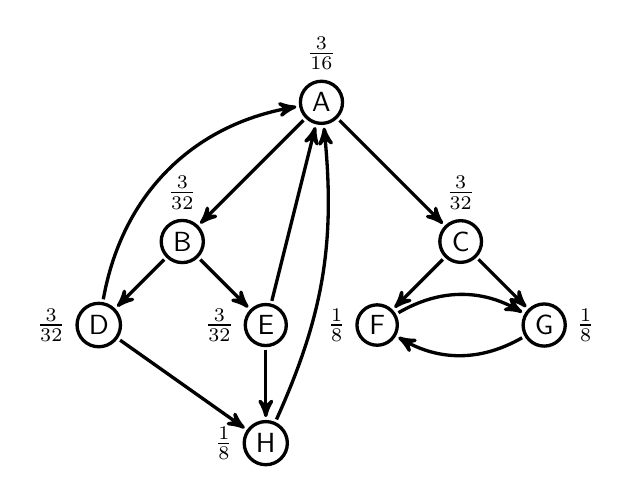
\begin{tikzpicture}[node distance=1.5cm]
                \node[vertex]       (A) [label={above:$\frac{3}{16}$}]                  						{\textsf{A}};
                \node[vertex]       (B) [below left of=A,node distance=2.5cm,label={above:$\frac{3}{32}$}]   {\textsf{B}};
                \node[vertex]       (C) [below right of=A,node distance=2.5cm,label={above:$\frac{3}{32}$}]  {\textsf{C}};
                \node[vertex]       (D) [below left of=B,label={left:$\frac{3}{32}$}]   						{\textsf{D}};
                \node[vertex]       (E) [below right of=B,label={left:$\frac{3}{32}$}]  						{\textsf{E}};
                \node[vertex]       (F) [below left of=C,label={left:$\frac{1}{8}$}]   						{\textsf{F}};
                \node[vertex]       (G) [below right of=C,label={right:$\frac{1}{8}$}]  					{\textsf{G}};
                \node[vertex]       (H) [below of=E,label={left:$\frac{1}{8}$}]  							{\textsf{H}};

                \path [very thick,->]  	(A) edge []             node [] {} (B)
                                        (A) edge []             node [] {} (C)
                                        (B) edge []             node [] {} (D)
                                        (B) edge []             node [] {} (E)
                                        (C) edge []             node [] {} (F)
                                        (C) edge []             node [] {} (G)
                                        (D) edge [bend left=35]             node [] {} (A)
                                        (D) edge []             node [] {} (H)
                                        (E) edge []             node [] {} (A)
                                        (E) edge []             node [] {} (H)
                                        (F) edge [bend left]             node [] {} (G)
                                        (G) edge [bend left]             node [] {} (F)
                                        (H) edge [bend right=15]             node [] {} (A);
        \end{tikzpicture} \\
        Initialisation & First Iteration \\
    \end{tabular}


    In this diagram: A network in which regular PageRank would let \textsf{F} and \textsf{G} behave as sinks and the first iteration of scaled PageRank with $s=\frac{1}{2}$.
\end{center}


\section{Network Models}

\subsection{Random Graphs}

\paragraph{Erdős–Rényi Graphs}

An \textit{Erdős–Rényi graph} $G(n,p)$ takes two parameters: $n$, the order of the graph to be generated, and $p$, the probability for an edge to exist.

\begin{center}
    \begin{tabular}{|l|l|}
        Properties & \\ \hline
        Mean degree & $c = (n-1) \cdot p$ \\
        Degree distribution & $P(deg_G(v) = k) = \frac{c^k}{k!}e^{-c}$ \\
        Clustering coefficient & $C = \frac{c}{n-1} = p$ \\
        Diameter & $\ell = \frac{\ln n}{\ln c}$ \\
        Fraction of vertices in GCC & $S = 1 - e^{-cS}$ \\
        GCC critical average degree & $c=1$ \\
    \end{tabular}
\end{center}
\smallskip

Erdős–Rényi graphs have a giant connected component if their average degree is at least one.
Their diameter is relatively small and their clustering is low in comparison to empirical networks.

\subsection{Small-World Networks}

Recall the small-world property from~\cref{sec:small-world} where graphs with this property have small distance but a high clustering coefficient.

To generate a small-world graph with $n$ nodes, a number $x$, and probability $p$ we follow these steps:
\begin{enumerate}
    \item Start with a ring with $n$ nodes and connect every node with its $\frac{x}{2}$ neighbours to each side. Thus, every node has degree $x$.
    \item Go through each edge and reconnect it with probability $p$: Choose a new node for one end of the edge.
\end{enumerate}

A second way of generating these networks is adding new random edges with probability $p$, rather than changing the old ones, in the initial ring. This results in the ring structure plus a random graph.

\begin{center}
    \begin{tabular}{|l|l|}
        Properties & \\ \hline
        Mean degree & $c = xp$ \\
        Degree distribution & $P(deg_G(v) = k) = e^{-xp}\frac{(xp)^{k-x}}{(k-x)!}$ \\
        Clustering coefficient & $C = \frac{3(x-2)}{4(x-1)}$ (if $p = 0$)\\
        Diameter & $\ell = \frac{n}{2x}$ \\
    \end{tabular}
\end{center}

\subsection{The Configuration Model}

The \emph{configuration model} is a random graph model with two parameters: $G(n,\vec{k})$, where $\vec{k}$ is a sequence of degrees, one for each node.
There are two ways to generate a graph with the configuration model.

Approach 1 is \emph{probabilistic links}:
Calculate the probability that a link between nodes $i$ and $j$ exists: $p_{i,j}=\frac{k_i k_j}{2m}=\frac{k_i k_j}{\sum_{l=1}^n k_l}$.
Then fill the adjacency matrix with $1$ or $0$ correspondingly.
Approach 2: We add stubs equal to the degree in the degree sequence and repeatedly connect two stubs randomly.

The graph has a giant connected component if the condition $\langle k^2 \rangle -2 \langle k  \rangle > 0$ is fulfilled.
\begin{center}
    \begin{tabular}{|l|l|}
        Properties & \\ \hline
        Mean degree & $?$ \\
        Degree distribution & Specified \\
        Clustering coefficient & $C = \frac{1}{n} \frac{(\langle k^2 \rangle - \langle k \rangle)^2}{\langle k \rangle^3}$ \\
        Diameter & $\ell = \O(\log n)$ \\
    \end{tabular}
\end{center}

\subsection{The Barabási-Albert Model}

We introduce the \emph{scale-free property} which is also called the \emph{power-law}.
The functional relationship between the node degree $x$ and the frequency $f$ is $f(x)=a x^{-k}$.
This results in many nodes with low degree and few nodes with high degree.
The distribution follows the principle of ``the rich get richer''.

The \emph{Barabási-Albert model} generates scale-free graphs.
Generation is done in two phases:
\begin{enumerate}
    \setcounter{enumi}{-1}
    \item Start with $m_0$ nodes and connect them arbitrarily, such that every node has at least one link.
    \item Growth step: At each timestep add a new node and connect it with $m (\leq m_0)$ links that connect to $m$ nodes already in the network.
    \item Preferential attachment: The probability $\Gamma(k)$ that a link of the new node connects to node $i$ depends on the degree $k_i$: $\Gamma(k_i) = \frac{k_i}{\sum_j k_j}$
\end{enumerate}

Many real-world networks are scale-free but many are also not.

\subsection{Network Robustness}

We now look at the robustness of networks to node and edge failures.

\begin{halfboxl}
    \paragraph{Robustness of Erdős–Rényi Graphs}
    On the right, we approximate the share of vertices remaining in the giant component of Erdős–Rényi graphs when successively \textcolor{bluishgreen}{removing random vertices} and when \textcolor{reddishpurple}{always removing the vertex with the highest degree}.
    We observe that succesively removing vertices of  large degree very quickly breaks the network, and that this type of network isn't robust against random attacks either.
\end{halfboxl}%
\begin{halfboxr}
    \vspace{-\baselineskip}
    \begin{center}
        \begin{tikzpicture}
            \draw[->] (0,0) -- (4,0) node[above right] {\begin{tabular}{c} \# of removed \\ vertices \end{tabular}};
                \draw[->] (0,0) -- (0,3) node[above right] {\begin{tabular}{c} \% of vertices in \\ giant component \end{tabular}};
                \draw[color=bluishgreen] plot[
                                mark=none,
                                samples=100,
                                domain=0:4,
                        ] ({\x},{-1/(1+exp(-((\x*2)-6)))*2.3+2.5});
                \draw[color=reddishpurple] plot[
                                mark=none,
                                samples=100,
                                domain=0:4,
                        ] ({\x},{-1/(1+exp(-((\x*4)-6)))*2.3+2.5});
        \end{tikzpicture}
    \end{center}
\end{halfboxr}%
\vspace{-20pt}

\paragraph{Robustness of Scale-Free Networks}
Scale-free networks on the other hand are quasi-immune to random attacks as the only real way of breaking them up is to hit the hubs, which is unlikely as they are comparatively few.
However, they are thus much more susceptible to precise attacks on the hubs.
We can explain this using the \emph{Molloy-Reed criterion} below.

\begin{defi}{Molloy-Reed Criterion}
    The \textit{Molloy-Reed criterion} states that a graph has a giant component if $\frac{\langle k^2 \rangle}{\langle k \rangle} \ge 2$.
\end{defi}

\section{Mesoscopic Structure}

\subsection{Detecting Communities}

\paragraph{Hierarchical Clustering}

\textit{Hierarchical clustering} is a technique used to arrange nodes of a graph in a so-called \textit{dendrogram} (see examples) such that vertices which are more likely to be in the same community are connected earlier on. The advantage is that here, we can first analyse the structure of a graph \textit{before} deciding where to actually split the graph into communities. In the following, we present two heuristics which generate such dendrograms.

\begin{thirdboxl}
    \begin{center}
        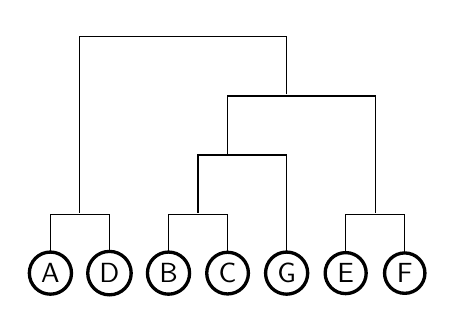
\begin{tikzpicture}[node distance=0.75cm,shorten >= 0pt,shorten <= -3pt]
            \node[]       (A) at (0,0)                    {\textsf{A}};
            \node[]       (D) at (0.75,0)                 {\textsf{D}};
            \node[]       (B) at (1.5,0)                  {\textsf{B}};
            \node[]       (C) at (2.25,0)                 {\textsf{C}};
            \node[]       (G) at (3,0)                    {\textsf{G}};
            \node[]       (E) at (3.75,0)                 {\textsf{E}};
            \node[]       (F) at (4.5,0)                  {\textsf{F}};

            \node[] (AD) at (0.375,0.75)        {};
            \node[] (BC) at (1.875,0.75)        {};
            \node[] (EF) at (4.125,0.75)        {};
            \node[] (BCG) at (2.25,1.5)         {};
            \node[] (BCGEF) at (3,2.25)         {};
            \node[] (ALL) at (2.25,3)           {};

            \draw  (A) |- (AD.center);
            \draw  (D) |- (AD.center);
            \draw  (B) |- (BC.center);
            \draw  (C) |- (BC.center);
            \draw  (E) |- (EF.center);
            \draw  (F) |- (EF.center);
            \draw  (BC) |- (BCG.center);
            \draw  (G) |- (BCG.center);
            \draw  (BCG) |- (BCGEF.center);
            \draw  (EF) |- (BCGEF.center);
            \draw  (AD) |- (ALL.center);
            \draw  (BCGEF) |- (ALL.center);

            \node[vertex]       (A) at (0,0)                    {\textsf{A}};
            \node[vertex]       (D) at (0.75,0)                 {\textsf{D}};
            \node[vertex]       (B) at (1.5,0)                  {\textsf{B}};
            \node[vertex]       (C) at (2.25,0)                 {\textsf{C}};
            \node[vertex]       (G) at (3,0)                    {\textsf{G}};
            \node[vertex]       (E) at (3.75,0)                 {\textsf{E}};
            \node[vertex]       (F) at (4.5,0)                  {\textsf{F}};
        \end{tikzpicture}
    \end{center}
\end{thirdboxl}%
\begin{thirdboxm}
    \begin{center}
        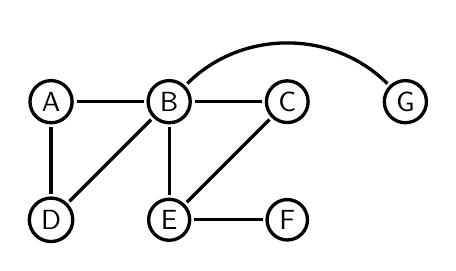
\begin{tikzpicture}[node distance=1.5cm]
            \node[vertex]       (A) []                  {\textsf{A}};
            \node[vertex]       (B) [right of=A]        {\textsf{B}};
            \node[vertex]       (C) [right of=B]        {\textsf{C}};
            \node[vertex]       (D) [below of=A]        {\textsf{D}};
            \node[vertex]       (E) [right of=D]        {\textsf{E}};
            \node[vertex]       (F) [right of=E]        {\textsf{F}};
            \node[vertex]       (G) [right of=C]        {\textsf{G}};

            \path [very thick]  	(A) edge []             node [] {} (B)
                                    (A) edge []             node [] {} (D)
                                    (B) edge []             node [] {} (C)
                                    (B) edge []             node [] {} (D)
                                    (B) edge []             node [] {} (E)
                                    (B) edge [bend left=45]             node [] {} (G)
                                    (C) edge []             node [] {} (E)
                                    (E) edge []             node [] {} (F);
        \end{tikzpicture}
    \end{center}
\end{thirdboxm}%
\begin{thirdboxr}
    \begin{center}
        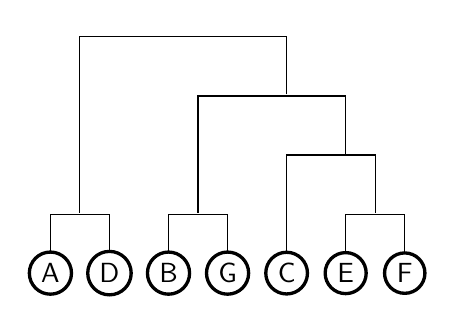
\begin{tikzpicture}[node distance=0.75cm,shorten >= 0pt,shorten <= -3pt]
            \node[]       (A) at (0,0)                  {\textsf{A}};
            \node[]       (D) at (0.75,0)       {\textsf{D}};
            \node[] (AD) at (0.375,0.75)        {};
            \node[]       (B) at (1.5,0)         {\textsf{B}};
            \node[]       (G) at (2.25,0)         {\textsf{G}};
            \node[] (BG) at (1.875,0.75)        {};
            \node[]       (C) at (3,0)         {\textsf{C}};
            \node[]       (E) at (3.75,0)         {\textsf{E}};
            \node[]       (F) at (4.5,0)         {\textsf{F}};
            \node[] (EF) at (4.125,0.75)        {};
            \node[] (CEF) at (3.75,1.5)        {};
            \node[] (BGCEF) at (3,2.25)        {};
            \node[] (ALL) at (2.25,3)        {};
            \draw  (A) |- (AD.center);
            \draw  (D) |- (AD.center);
            \draw  (B) |- (BG.center);
            \draw  (G) |- (BG.center);
            \draw  (E) |- (EF.center);
            \draw  (F) |- (EF.center);
            \draw  (C) |- (CEF.center);
            \draw  (EF) |- (CEF.center);
            \draw  (BG) |- (BGCEF.center);
            \draw  (CEF) |- (BGCEF.center);
            \draw  (AD) |- (ALL.center);
            \draw  (BGCEF) |- (ALL.center);
            \node[vertex]       (A) at (0,0)                  {\textsf{A}};
            \node[vertex]       (D) at (0.75,0)       {\textsf{D}};
            \node[] (AD) at (0.375,0.75)        {};
            \node[vertex]       (B) at (1.5,0)         {\textsf{B}};
            \node[vertex]       (G) at (2.25,0)         {\textsf{G}};
            \node[] (BG) at (1.875,0.75)        {};
            \node[vertex]       (C) at (3,0)         {\textsf{C}};
            \node[vertex]       (E) at (3.75,0)         {\textsf{E}};
            \node[vertex]       (F) at (4.5,0)         {\textsf{F}};
            \node[] (EF) at (4.125,0.75)        {};
            \node[] (CEF) at (3.75,1.5)        {};
            \node[] (BGCEF) at (3,2.25)        {};
            \node[] (ALL) at (2.25,3)        {};
        \end{tikzpicture}
    \end{center}
\end{thirdboxr}
\begin{tightcenter}
    In this diagram: A graph $G$ (middle) and two dendrograms, one obtained by the Ravasz algorithm (left), and one obtained by the Girvan-Newman Algorithm (right).
\end{tightcenter}

\medskip

\begin{algo}{Ravasz}
    \textbf{Input:} A graph $G=(V(G), E(G))$.\\
    \textbf{Output:} A dendrogram for $G$.
    \tcblower
    \begin{enumerate}
            \item Set up the similarity matrix $X^0 \in \mathbb{R}^{|V(G)|\times|V(G)|}$ $\Forall v,w \in V(G)$:
                \[
                    X^0_{vw}=\frac{|N_G(v,w)| + \Theta(A_{vw})}{\min(k_v,k_w) + 1 - \Theta(A_{vw})},
                \]
                {\footnotesize{}
                where $\Theta$ is the \emph{Heaviside function}: $\Theta(x) = 0$ if $x \leq 0$, $\Theta(x) = 1$ otherwise.}
            \item Assign every node to a community of its own.
            \item While there is more than one community:
                    \begin{enumerate}
                            \item For all pairs of communities $A$ and $B$, compute the \textit{average linkage similarity} given by:
                                    \[
                                        als(A,B) = \frac{1}{|A|\cdot|B|}\sum_{a\in A} \sum_{b \in B} X^0_{ab}.
                                    \]
                                {\footnotesize{}(This is just the average pairwise similarity between vertices in $A$ and $B$.)}
                            \item Merge the pair of clusters where $als(A,B)$ is maximal.
                    \end{enumerate}
            \item Generate the dendrogram in the order in which the communities were merged, i.e.\ if two singleton communities are merged, they are connected at the lowest step in the dendrogram.
    \end{enumerate}
\end{algo}

\begin{algo}{Girvan-Newman}
\textbf{Input:} A graph $G=(V(G), E(G))$.\\
\textbf{Output:} A dendrogram for $G$.
\tcblower
\begin{enumerate}
    \item While $E(G) \neq \varnothing:$
    \begin{enumerate}
        \item For every edge, compute $vw \in E(G)$ the \textit{link betweenness} $L_{vw}$ (analogous to node betweenness centrality, but for links).
                \item Remove the edge with $\max L_{vw}$.
                            If there are multiple, choose one randomly.
    \end{enumerate}
    \item Generate the dendrogram in the reverse order in which the edges were removed, i.e.\ if an edge is removed last, the corresponding vertices are connected at the lowest step of the dendrogram.
\end{enumerate}
\end{algo}

The Ravasz algorithm is called an \textit{agglomerative algorithm} as we successively merge vertices into larger and larger communities, while the Girvan-Newman algorithm is a \textit{divisive algorithm}, where we break up the network successively and observe which parts stay connected the longest.
By varying the heuristics we use we can obviously obtain different results, for example by instead of computing the average linkage similarity in the Ravasz Algorithm, choosing the communities with the largest overall linkage.

\subsection{Cutting a Dendrogram}

There are multiple heuristics for cutting a dendrogram. For example, we can for try to split such that the coverage, i.e.\ the ratio between in-community edges versus total number of edges is maximised. Another more complex method is to maximise the modularity of a partition.

\subsection{Modularity}

The \emph{modularity of a partition} is given by
\[
    M= \sum_{c=1}^p \left(\frac{|E_c(G)|}{|E(G)|} - \left(\frac{k_c}{2\cdot|E(G)|}\right)^2 \right),
\]
where $k_c$ is the sum of the degrees within a community $c$ and $E_c(G)$ are the edges.

\begin{algo}{Greedy Modularity Maximisation}
    \textbf{Input:} A graph $G$ and a corresponding dendrogram. \\
    \textbf{Output:} A partition of $V(G)$.
    \tcblower
    \begin{enumerate}
            \item Consider the partition $P$ where every vertex is an individual community.
            \item Compute $M$, the modularity of the current partition.
            \item While $|P| > 1$:
                \begin{enumerate}
                        \item Store $M$.
                        \item For every one merge of the dendrogram, compute the change $\Delta M$ of the modularity.
                        \item Follow the merge where $\Delta M$ is the largest.
                        \item Compute $M$, the modularity of the current partition.
                \end{enumerate}
            \item Return the visited partition of the largest modularity.
    \end{enumerate}
\end{algo}

The modularity of a partition can also be computed in another way: $$M = \sum_c \left(e_{cc} - k_c^2\right),$$ where for every community $c$, $e_{cc}$ is the ratio of in-community edges to all edges, while $k_c$ is the ratio of the sum of vertex degrees in $c$ to the overall sum of vertex degrees ($2m$).

\paragraph{Label Propagation}
\textit{Label propagation} is a very fast and local algorithm to detect communities.
First, every vertex is initialised to have a unique label.
Then, in every step (and generally in a random order), every vertex is assigned the label of which it has the most neighbours.
Ties are resolved by a random choice.
This algorithm can find any number of communities of any size and is very fast.
However, its results are not unique and it can get stuck in oscillations, for example in bipartite subgraphs.

\subsection{Judging the Quality of Detected Communities}

\paragraph{Rand Index}
Assume you are given two partitions $X$ and $Y$ of a same graph, where $X$ is the actual partition and $Y$ is one obtained by some algorithm, the \emph{Rand index} $\mathcal{R}$ is a measure of how well the computed partition fares compared to the actual one.
It is given by
\[
    \mathcal{R} = \frac{n_{00} + n_{11}}{n_{00} + n_{01} + n_{10} + n_{11}}.
\]

\begin{center}
    \begin{tabular}{cl}
        $n_{00}$: & number of pairs vertices in different communities in both $X$ and $Y$. \\
        $n_{01}$: & number of pairs vertices in different communities in $X$ but not $Y$. \\
        $n_{10}$: & number of pairs vertices in same communities in $X$ but not $Y$. \\
        $n_{11}$: & number of pairs vertices in same communities in both $X$ and $Y$. \\
    \end{tabular}
\end{center}

\paragraph{Homophily}
Given a graph and two types of labels with occurring probabilities $p$ and $1-p$ respectively, the real probability for an edge to have both its endpoints of the same label is $p^2 + (1-p)^2$, while the probability for an inter-label edge is $2p(1-p)$.
We say that a network tends to show \textit{homophily} if the share of inter-label edges is significantly less than $2p(1-p)$.
On the other hand, if it is significantly larger, we talk about \textit{heterophily}.

In general, modularity is a good indicator for homophily.

Two influencing factors for homophily in social networks are \textit{influence} and \textit{selection}: people tend to become more like the people around them and people tend to connect more to people which are already like themselves.

\paragraph{Degree Assortativity}
The \textit{degree assortativity} of a graph is given by:
\[
    r = \frac{S_1S_e - S_2^2}{S_1S_3 -S_2^2},
\]
where $S_e = 2 \cdot \sum_{vw \in E(G)} k_vk_w$ and for $p \in \Set{1,2,3}$, $S_p = \sum_{v \in V(G)} k_v^p$.

A network with high degree assortativity ($r>0$) tends to have a structure where hubs connect to hubs and low degree vertices tend to connect to low degree vertices.
We call this a \textit{core-periphery} structure.
In a network with high degree \textit{disassortativity} ($r<0$), hubs tend to connect to small degree vertices and vice-versa.
Erdős–Rényi and Barabási-Albert graphs in general have $r \approx 0$.

\paragraph{Degree Correlation Function}
The \textit{degree correlation function} $k_{nn}(k)$ returns the average degree of an arbitrary node we reach by selecting a random node of degree $k$ and following a random link, or:
\[
    k_{nn}(k) = \sum_{k'}k'\cdot P(k'|k).
\]
\vspace{-2\baselineskip} % to fit infection models on page 12

\paragraph{Friendship Paradox}
\label{par:friendshipparadox}
The \emph{friendship paradox} states that most vertices have less neighbours on average than their neighbours.
Given a random graph with average degree $\langle k \rangle$ and selecting a random vertex, we can show that his neighbours have $\frac{\langle k^2 \rangle}{\langle k \rangle}$ neighbours on average.

\section{Dynamics and Spreading}

Networks can be used to model spreading, for example how diseases spread in a population.
The population is modelled by a graph of people as nodes and interactions as vertices.

\subsection{Infection Models}

The \textit{characteristic time} of a given model is the number of steps needed to infect about $\frac{1}{e} \approx 36\%$ of the nodes.
The \textit{basic reproductive number} is the average number of individuals an infected node will infect before recovering in a completely susceptible population.

\begin{minipage}[t]{0.475\textwidth}
    \paragraph{SIS Model}
    \begin{center}
        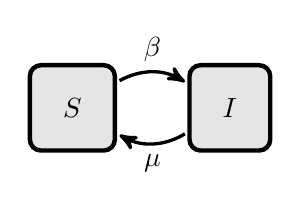
\begin{tikzpicture}
            \node[box]       (S) []             {$S$};
            \node[box]       (I) [right of=S]   {$I$};
            \path [very thick,->]  	(S) edge [bend left]    node [above] {$\beta$}  (I)
                                    (I) edge [bend left]    node [below] {$\mu$}    (S);
        \end{tikzpicture}

        \begin{tabular}{c|c}
            Characteristic Time & $\tau = \frac{1}{\mu \cdot (R_0 - 1)}$ \\
            BRN & $R_0 = \frac{\beta \langle k \rangle}{\mu}$ \\
            Spreading Rate & $\lambda = \frac{\beta}{\mu}$ \\
            Epidemic Threshold & $\lambda_c = \frac{\langle k \rangle}{\langle k^2 \rangle}$ \\
        \end{tabular}
    \end{center}
    If $R_0 > 1$, then every node infects at least one other before becoming susceptible again.
    The epidemic is endemic.
    In terms of the spreading rate, the epidemic spreads if $\lambda > \lambda_c$.

    If $R_0 < 1$, then every nodes infects less than one other before becoming susceptible again. The epidemic dies out.
    In terms of the spreading rate, the epidemic dies out if $\lambda < \lambda_c$.

    Observe that for power law networks, $\lambda_c$ diverges when $n \to \infty$, which implies that in these networks, even very slow viruses can spread successfully there.

    In this model, either the infection dies out, or after enough time some fraction of the population (given by $1-\frac{\mu}{\beta \langle k \rangle}$) is infected.
\end{minipage}\hfil{\color[gray]{0.7}\vline}\hfil%
\begin{minipage}[t]{0.475\textwidth}
    \vspace{-\baselineskip}
    \paragraph{SI Model}
    \begin{center}
        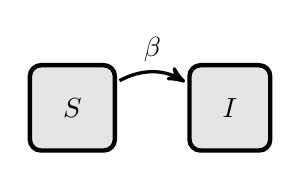
\begin{tikzpicture}
            \node[box]       (S) []            {$S$};
            \node[box]       (I) [right of=S]  {$I$};
            \path [very thick,->]  (S) edge [bend left]    node [above] {$\beta$}   (I);
        \end{tikzpicture}

        \begin{tabular}{c|c}
            Characteristic Time & $\tau = \frac{1}{\beta \langle k \rangle}$ \\
        \end{tabular}
    \end{center}
    In this model, all nodes become infected given enough time.

    \paragraph{SIR Model}
    \begin{center}
        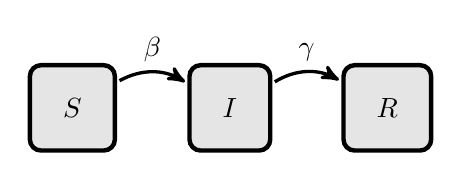
\begin{tikzpicture}
                    \node[box]       (S) []              {$S$};
                    \node[box]       (I) [right of=S]              {$I$};
                    \node[box]       (R) [right of=I]              {$R$};
                    \path [very thick,->]  	(S) edge [bend left]             node [above] {$\beta$} (I)
                                            (I) edge [bend left]             node [above] {$\gamma$} (R);
        \end{tikzpicture}
    \end{center}

    In this model, all nodes recover given enough time.
    \paragraph{SIRS Model}
    \begin{center}
        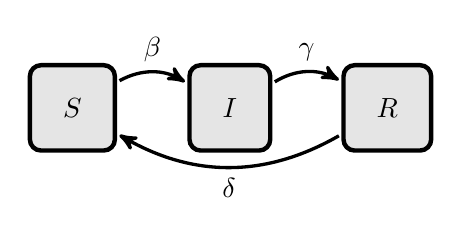
\begin{tikzpicture}
                    \node[box]       (S) []              {$S$};
                    \node[box]       (I) [right of=S]              {$I$};
                    \node[box]       (R) [right of=I]              {$R$};
                    \path [very thick,->]  	(S) edge [bend left]             node [above] {$\beta$} (I)
                                            (I) edge [bend left]             node [above] {$\gamma$} (R)
                                            (R) edge [bend left=30]          node [below] {$\delta$} (S);
        \end{tikzpicture}
    \end{center}
    Analytically not solvable.
\end{minipage}

\begin{center}
    \begin{tabular}{c|l}
        Legend & \\ \hline
        $S$ 		& Set of susceptible nodes \\
        $I$ 		& Set of infected nodes \\
        $R$ 		& Set of recovered/removed nodes \\
        $\beta \in [0,1]$  		& In each step, likelihood of an infected node infecting one of its neighbours. \\
        $\mu \in [0,1]$  		& In each step, likelihood of an infected node becoming susceptible again. \\
        $\gamma \in [0,1]$  	& In each step, likelihood of an infected node recovering. \\
        $\delta \in [0,1]$  	& In each step, likelihood of a recovered node to become susceptible again. \\
    \end{tabular}
\end{center}

\paragraph{Vaccination Strategies}

An interesting questions is, ``how can we stop the spread of infections in real networks effectively and at a limited cost?''
Three approaches have been discussed in the lecture:
\begin{itemize}
    \item Random vaccination: Ineffective, as power-law networks are very robust against random node attacks.
    \item Hub vaccination: Theoretically ideal as it would break the network. Impractical however, as this requires knowledge of hubs.
    \item Random neighbour vaccination: Sample the population and vaccinate, for each node, a random neighbour (see \nameref{par:friendshipparadox}).
        Balances the two previous approaches.
\end{itemize}

\subsection{Cascading Behaviour}

In this part, we discuss the emergence of group behaviour based on individual thresholds.
For a population given by $P = \Set{1,\dots,n}$, let $\theta(i) = x, i \in P$ be the behaviour threshold for individual $i$, meaning $i$ joins a certain group behaviour only if at least $x$ others are already participating.

Let $f(x)$ be the corresponding frequency distribution while $F(x)$ corresponds to the cumulative distribution.
Denoting discrete time steps as $t \in 1,2,\dots$, let $r(t)$ denote the number of participants at time $t$.
We can then calculate $r(t+1) := F(r(t))$: the number of people whose threshold is below the number of current participants will join in the next time step.

An \textit{equilibrium} is reached once $r(t) = r(t+1)$: when no new people join the behaviour, either because they have a higher threshold or because everyone is participating.

If we now assume that $f$ is a normal distribution (pertinent, as in reality this is often approximately the case), we often observe that there is a tipping point tied to the standard deviation of $f$.
Below it, only very few participate, while above it, almost everyone participates in the behaviour.

\paragraph{Network Behaviour}

Assume a given network $G$, in which every node can choose between two alternatives, $A$ and $B$ such that, for every edge $vw \in E(G)$, if $v$ and $w$ both chose $A$ or $B$, they get both payoffs $a > 0$ or $b > 0$ respectively, whereas if they chose different alternatives, they both get payoff 0.
Initially, everybody uses alternative $B$, while a select few choose $A$ for some reason.
Then in a given time step every $v \in V(G)$ would adopt $A$ if $$p \cdot |N_G(v)| \cdot a \ge (1-p) \cdot |N_G(v)| \cdot b,$$ where $p$ is the share of neighbours having adopted $A$ (simple payoff maximisation).
The formula can be shortened to $p \ge \frac{b}{a + b}$.

We call it a \textit{complete cascade} if after a certain number of time steps, all nodes switch from $B$ to $A$.
A complete cascade can be stopped by a $B$ cluster of density at least $1 - p$: a set of nodes such that every node in it has selected $B$ and has at least a fraction of $p$ neighbours who have also selected $B$.
It is easy to prove that only such clusters can stop a complete cascade.

\subsection{Weak Ties}

In this section, we discuss a discovery by Mark Granovetter about job acquisition.
He observed that although many people got their jobs through social contacts, most didn't come through close friends (strong ties), but rather through acquaintances (weak ties).

\paragraph{Triadic Closure}
\textit{Triadic closure} is the term used to describe the phenomenon in social networks in which nodes with a shared neighbour have a stronger than average likelihood of in turn developing a shared link, which in turn provides both with social opportunities.

\paragraph{Local Bridge}
A \textit{local bridge} is an edge in a network such that its endpoints have no common neighbours.

\paragraph{Strong Triadic Closure Property} The \textit{STCP} (which is actually an \textbf{assumption}) states that if a vertex has a strong tie to two other vertices, then these two share a tie, either weak or strong.

\begin{halfboxl}
    It implies that every local bridge must have one weak tie.
    A proof by contradiction is drawn on the right.
    Two strong ties would imply a weak tie between the other vertices, thus the local bridge isn't a bridge anymore.

    Further, the STCP implies that weak ties are those that connect more distant parts of a network and that removing them is more likely to destroy a network than removing strong ties.
\end{halfboxl}%
\begin{halfboxr}
    \vspace{-\baselineskip}
    \begin{center}
        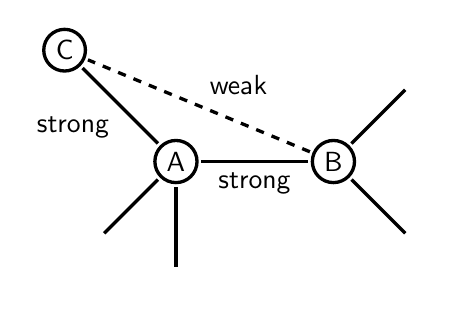
\begin{tikzpicture}
                    \node[vertex]  (A) []                      {\textsf{A}};
                    \node[vertex]  (B) [right of=A]            {\textsf{B}};
                    \node[vertex]  (C) [above left of=A]       {\textsf{C}};
                    \node[]  (a1) [below left of=A,node distance=1.5cm]         {};
                    \node[]  (a2) [below of=A,node distance=1.5cm]              {};
                    \node[]  (b1) [below right of=B,node distance=1.5cm]       {};
                    \node[]  (b2) [above right of=B,node distance=1.5cm]       {};

                    \path [very thick]  	(A) edge []             node [below] {\textsf{strong}} (B)
                                            (A) edge []             node [below left] {\textsf{strong}} (C)
                                            (B) edge [dashed]          node [above right] {\textsf{weak}} (C)
                                            (A) edge []             node [] {} (a1)
                                            (A) edge []             node [] {} (a2)
                                            (B) edge []             node [] {} (b1)
                                            (B) edge []             node [] {} (b2);
        \end{tikzpicture}

        In this diagram: A local bridge that isn't one.
    \end{center}
\end{halfboxr}

This has been observed across a variety of networks, and is among others a nice property to reduce the spread of infections as weak ties are less likely to transmit them.

\section{Link Prediction}

In this section we discuss how we can, given a network, predict which new links might form in the future and which tools we have to predict these.

\subsection{Neighbourhood Approaches}

A simple method is to assign pairs of vertices scores based on their neighbourhoods.
These scores are convenient as they are easy to understand and easy to implement as they only require local information.
However, they are less accurate than other, more complex techniques.

\begin{halfboxl}
    \vspace{-\baselineskip}
    \begin{defi}{Common Neighbours}
        The \textit{common neighbour score} returns, for two $v,w \in V(G)$, the number of neighbours they have in common:
        \[
            S_{CN}(v,w)=|N_G(v) \cap N_G(w)|.
        \]
    \end{defi}

    \begin{defi}{Jaccard}
        The \textit{Jaccard score} for two $v,w \in V(G)$ is given by:
        \[
            S_J(v,w) = \frac{|N_G(v) \cap N_G(w)|}{|N_G(v) \cup N_G(w)|}.
        \]

        \footnotesize{}
        Informally, we measure how many of their neighbours they have in common compared to their overall number of neighbours.
    \end{defi}
\end{halfboxl}%
\begin{halfboxr}
    \vspace{-\baselineskip}
    \begin{defi}{Adamic-Adar}
        The \textit{Adamic-Adar score} values shared neighbours of small degree more.
        Formally: \[
            S_{AA}(v,w) = \sum_{u \in N_G(v) \cap N_G(w)} \frac{1}{\log |N_G(u)|}.
        \]

        \footnotesize{}
        For example, two people who regularly visit the same small bar are much more likely to meet than two people who regularly attend a same large concert venue.
    \end{defi}

    \begin{defi}{Preferential Attachment}
        The \textit{preferential attachment score} assumes that two hubs are likely to become connected at some point:
        \[
            S_{PA}(v,w) = |N_G(v)||N_G(w)|.
        \]
    \end{defi}
\end{halfboxr}

\subsection{Path Approaches}

A somewhat more sophisticated approach would be to use path information to predict new links. However, even these are not very good and computationally very expensive.

\begin{defi}{Distance}
    The \textit{distance score} for two vertices $v,w \in V(G)$ is the negation of the distance of the two:
    \[
        S_D(v,w) = -d(v,w).
    \]
\end{defi}

\begin{defi}{Katz Similarity}
    The \textit{Katz similarity score} sums over all paths of length $\ell$, where $\beta \in [0,1]$:
    \[
        S_{KS}(v,w) = \sum_{\ell=1}^{\infty} \beta^\ell \left|\textsf{paths}_{vw}^{(\ell)}\right|.
    \]
    By tuning $\beta$, it is possible to adjust how much value to put on longer paths.
\end{defi}

More complex machine learning classifiers (logistic regression, SVMs, or NNs) yield much better results.
They are however much less transparent in their results.
Further, use of meta-data and community structures can yield improved results.

\section{Directed and Signed Networks}

\subsection{Directed Networks}

\paragraph{Triadic Census}
We can do a \emph{triadic census} that evaluates every vertex triple in a graph.
The result is a $T \in \N^{1 \times 16}$ vector, counting how often each of the 16 triads below occured.

\begin{center}
\setlength{\tabcolsep}{15pt}
    \begin{tabular}{cccc}
        \begin{tikzpicture}[node distance=1.5cm]
                \node[vertex]       (A) []                  {};
                \node[vertex]       (B) [below left of=A]   {};
                \node[vertex]       (C) [below right of=A]  {};
                \node[]       (D) [below of=A]  {};
        \end{tikzpicture} & 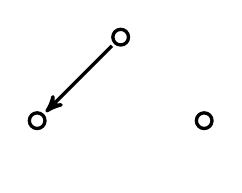
\begin{tikzpicture}[node distance=1.5cm]
                \node[vertex]       (A) []                  {};
                \node[vertex]       (B) [below left of=A]   {};
                \node[vertex]       (C) [below right of=A]  {};
                \node[]       (D) [below of=A]  {};
                \path [very thick,->]  	(A) edge []             node [] {} (B);
        \end{tikzpicture} & 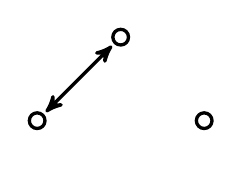
\begin{tikzpicture}[node distance=1.5cm]
                \node[vertex]       (A) []                  {};
                \node[vertex]       (B) [below left of=A]   {};
                \node[vertex]       (C) [below right of=A]  {};
                \node[]       (D) [below of=A]  {};
                \path [very thick,->]  	(A) edge [<->]             node [] {} (B);
        \end{tikzpicture} & 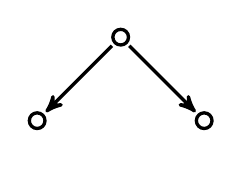
\begin{tikzpicture}[node distance=1.5cm]
                \node[vertex]       (A) []                  {};
                \node[vertex]       (B) [below left of=A]   {};
                \node[vertex]       (C) [below right of=A]  {};
                \node[]       (D) [below of=A]  {};
                \path [very thick,->]  	(A) edge []             node [] {} (B)
                                        (A) edge []             node [] {} (C);
        \end{tikzpicture} \\ 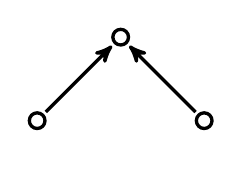
\begin{tikzpicture}[node distance=1.5cm]
                \node[vertex]       (A) []                  {};
                \node[vertex]       (B) [below left of=A]   {};
                \node[vertex]       (C) [below right of=A]  {};
                \node[]       (D) [below of=A]  {};
                \path [very thick,->]  	(B) edge []             node [] {} (A)
                                        (C) edge []             node [] {} (A);
        \end{tikzpicture} & 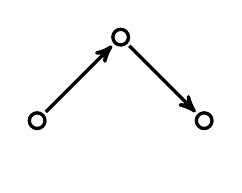
\begin{tikzpicture}[node distance=1.5cm]
                \node[vertex]       (A) []                  {};
                \node[vertex]       (B) [below left of=A]   {};
                \node[vertex]       (C) [below right of=A]  {};
                \node[]       (D) [below of=A]  {};
                \path [very thick,->]  	(B) edge []             node [] {} (A)
                                        (A) edge []             node [] {} (C);
        \end{tikzpicture} & 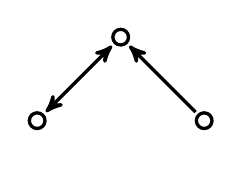
\begin{tikzpicture}[node distance=1.5cm]
                \node[vertex]       (A) []                  {};
                \node[vertex]       (B) [below left of=A]   {};
                \node[vertex]       (C) [below right of=A]  {};
                \node[]       (D) [below of=A]  {};
                \path [very thick,->]  	(B) edge [<->]             node [] {} (A)
                                        (C) edge []             node [] {} (A);
        \end{tikzpicture} & 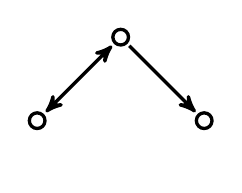
\begin{tikzpicture}[node distance=1.5cm]
                \node[vertex]       (A) []                  {};
                \node[vertex]       (B) [below left of=A]   {};
                \node[vertex]       (C) [below right of=A]  {};
                \node[]       (D) [below of=A]  {};
                \path [very thick,->]  	(B) edge [<->]             node [] {} (A)
                                        (A) edge []             node [] {} (C);
        \end{tikzpicture} \\ 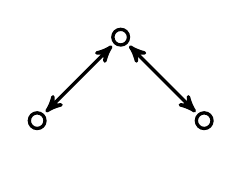
\begin{tikzpicture}[node distance=1.5cm]
                \node[vertex]       (A) []                  {};
                \node[vertex]       (B) [below left of=A]   {};
                \node[vertex]       (C) [below right of=A]  {};
                \node[]       (D) [below of=A]  {};
                \path [very thick,->]  	(A) edge [<->]             node [] {} (B)
                                        (A) edge [<->]             node [] {} (C);
        \end{tikzpicture} & 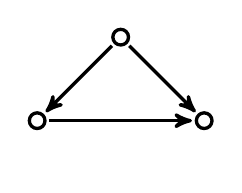
\begin{tikzpicture}[node distance=1.5cm]
                \node[vertex]       (A) []                  {};
                \node[vertex]       (B) [below left of=A]   {};
                \node[vertex]       (C) [below right of=A]  {};
                \node[]       (D) [below of=A]  {};
                \path [very thick,->]  	(A) edge []             node [] {} (B)
                                        (A) edge []             node [] {} (C)
                                        (B) edge []             node [] {} (C);
        \end{tikzpicture} & 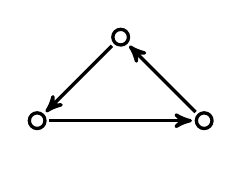
\begin{tikzpicture}[node distance=1.5cm]
                \node[vertex]       (A) []                  {};
                \node[vertex]       (B) [below left of=A]   {};
                \node[vertex]       (C) [below right of=A]  {};
                \node[]       (D) [below of=A]  {};
                \path [very thick,->]  	(A) edge []             node [] {} (B)
                                        (A) edge [<-]             node [] {} (C)
                                        (B) edge []             node [] {} (C);
        \end{tikzpicture} & 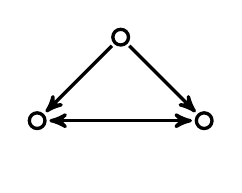
\begin{tikzpicture}[node distance=1.5cm]
                \node[vertex]       (A) []                  {};
                \node[vertex]       (B) [below left of=A]   {};
                \node[vertex]       (C) [below right of=A]  {};
                \node[]       (D) [below of=A]  {};
                \path [very thick,->]  	(A) edge []             node [] {} (B)
                                        (A) edge []             node [] {} (C)
                                        (B) edge [<->]             node [] {} (C);
        \end{tikzpicture} \\ 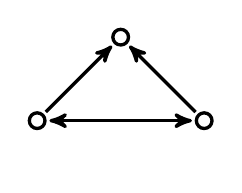
\begin{tikzpicture}[node distance=1.5cm]
                \node[vertex]       (A) []                  {};
                \node[vertex]       (B) [below left of=A]   {};
                \node[vertex]       (C) [below right of=A]  {};
                \node[]       (D) [below of=A]  {};
                \path [very thick,->]  	(A) edge [<-]             node [] {} (B)
                                        (A) edge [<-]             node [] {} (C)
                                        (B) edge [<->]             node [] {} (C);
        \end{tikzpicture} & 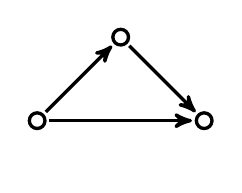
\begin{tikzpicture}[node distance=1.5cm]
                \node[vertex]       (A) []                  {};
                \node[vertex]       (B) [below left of=A]   {};
                \node[vertex]       (C) [below right of=A]  {};
                \node[]       (D) [below of=A]  {};
                \path [very thick,->]  	(A) edge [<-]             node [] {} (B)
                                        (A) edge []             node [] {} (C)
                                        (B) edge []             node [] {} (C);
        \end{tikzpicture} & 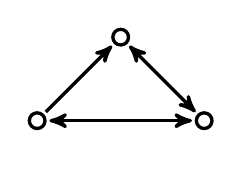
\begin{tikzpicture}[node distance=1.5cm]
                \node[vertex]       (A) []                  {};
                \node[vertex]       (B) [below left of=A]   {};
                \node[vertex]       (C) [below right of=A]  {};
                \node[]       (D) [below of=A]  {};
                \path [very thick,->]  	(A) edge [<-]             node [] {} (B)
                                        (A) edge [<->]             node [] {} (C)
                                        (B) edge [<->]             node [] {} (C);
        \end{tikzpicture} & 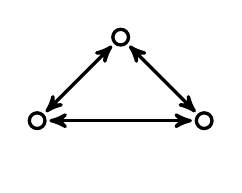
\begin{tikzpicture}[node distance=1.5cm]
                \node[vertex]       (A) []                  {};
                \node[vertex]       (B) [below left of=A]   {};
                \node[vertex]       (C) [below right of=A]  {};
                \node[]       (D) [below of=A]  {};
                \path [very thick,->]  	(A) edge [<->]             node [] {} (B)
                                        (A) edge [<->]             node [] {} (C)
                                        (B) edge [<->]             node [] {} (C);
        \end{tikzpicture}
    \end{tabular}

    In this table: The 16 triad motifs. All in all, there exist 64 realisations of these triads when distinguishing the vertices.
\end{center}


\paragraph{Flow Hierarchy}
\textit{Flow hierarchy} is a metric which measures how hierarchical a graph is, and is more nuanced than the binary hierarchical/not hierarchical.
Formally, the flow hierarchy is given by the size of the fraction of edges which are not part of a cycle:
\[
    h(G) = \frac{\sum_{e \in E(G)} \begin{cases}1, \text{ if } e \text{ is not in a cycle.}\\0, \text{ otherwise.} \end{cases}}{|E(G)|}.
\]

\begin{center}
    \begin{tabular}{cc}
        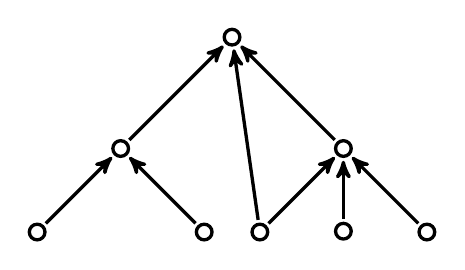
\begin{tikzpicture}[node distance=1.5cm]
                \node[vertex]       (A) []                  {};
                \node[vertex]       (B) [below left of=A,node distance=2cm]   {};
                \node[vertex]       (C) [below right of=A,node distance=2cm]  {};
                \node[vertex]       (D) [below left of=B]   {};
                \node[vertex]       (E) [below right of=B]  {};
                \node[vertex]       (F) [below left of=C]   {};
                \node[vertex]       (G) [below of=C,node distance=1.05cm]  {};
                \node[vertex]       (H) [below right of=C]  {};

                \path [very thick,<-]  	(A) edge []             node [] {} (B)
                                        (A) edge []             node [] {} (C)
                                        (A) edge []             node [] {} (F)
                                        (B) edge []             node [] {} (D)
                                        (B) edge []             node [] {} (E)
                                        (C) edge []             node [] {} (F)
                                        (C) edge []             node [] {} (G)
                                        (C) edge []             node [] {} (H);
        \end{tikzpicture} & 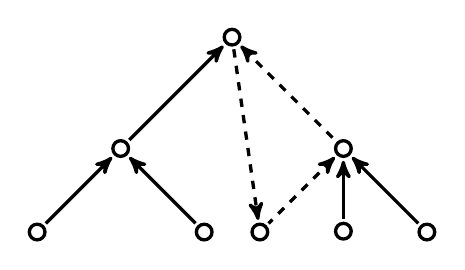
\begin{tikzpicture}[node distance=1.5cm]
                \node[vertex]       (A) []                  {};
                \node[vertex]       (B) [below left of=A,node distance=2cm]   {};
                \node[vertex]       (C) [below right of=A,node distance=2cm]  {};
                \node[vertex]       (D) [below left of=B]   {};
                \node[vertex]       (E) [below right of=B]  {};
                \node[vertex]       (F) [below left of=C]   {};
                \node[vertex]       (G) [below of=C,node distance=1.05cm]  {};
                \node[vertex]       (H) [below right of=C]  {};

                \path [very thick,<-]  	(A) edge []             node [] {} (B)
                                        (A) edge [dashed]             node [] {} (C)
                                        (A) edge [->,dashed]             node [] {} (F)
                                        (B) edge []             node [] {} (D)
                                        (B) edge []             node [] {} (E)
                                        (C) edge [dashed]             node [] {} (F)
                                        (C) edge []             node [] {} (G)
                                        (C) edge []             node [] {} (H);
        \end{tikzpicture} \\ \\
        hierarchical graph & non-hierarchical graph \\
        $h(G) = 1$ & $h(G) = \frac{5}{8}$ \\
    \end{tabular}
\end{center}


\subsection{Signed Networks}

There are four configurations of signed triangles to model three-way relations, some of them more stable than the others.
A network is called \textit{structurally balanced} if \textbf{all} its triangles are balanced (they are either of the first or the third type).

\begin{center}
    \begin{tabular}{cccc}
        \begin{tikzpicture}[node distance=1.75cm]
                \node[vertex]       (A) []                  {$\textsf{A}$};
                \node[vertex]       (B) [below left of=A]   {$\textsf{B}$};
                \node[vertex]       (C) [below right of=A]  {$\textsf{C}$};

                \path [very thick]  	(A) edge [bluishgreen] node [above left] {$\textcolor{bluishgreen}{+}$} (B)
                                        (A) edge [bluishgreen] node [above right] {$\textcolor{bluishgreen}{+}$} (C)
                                        (B) edge [bluishgreen] node [below] {$\textcolor{bluishgreen}{+}$} (C);
        \end{tikzpicture} & \begin{tikzpicture}[node distance=1.75cm]
                \node[vertex]       (A) []                  {$\textsf{A}$};
                \node[vertex]       (B) [below left of=A]   {$\textsf{B}$};
                \node[vertex]       (C) [below right of=A]  {$\textsf{C}$};

                \path [very thick]  	(A) edge [bluishgreen] node [above left] {$\textcolor{bluishgreen}{+}$} (B)
                                        (A) edge [bluishgreen] node [above right] {$\textcolor{bluishgreen}{+}$} (C)
                                        (B) edge [reddishpurple] node [below] {$\textcolor{reddishpurple}{-}$} (C);
        \end{tikzpicture} & \begin{tikzpicture}[node distance=1.75cm]
                \node[vertex]       (A) []                  {$\textsf{A}$};
                \node[vertex]       (B) [below left of=A]   {$\textsf{B}$};
                \node[vertex]       (C) [below right of=A]  {$\textsf{C}$};

                \path [very thick]  	(A) edge [bluishgreen] node [above left] {$\textcolor{bluishgreen}{+}$} (B)
                                        (A) edge [reddishpurple] node [above right] {$\textcolor{reddishpurple}{-}$} (C)
                                        (B) edge [reddishpurple] node [below] {$\textcolor{reddishpurple}{-}$} (C);
        \end{tikzpicture} & \begin{tikzpicture}[node distance=1.75cm]
                \node[vertex]       (A) []                  {$\textsf{A}$};
                \node[vertex]       (B) [below left of=A]   {$\textsf{B}$};
                \node[vertex]       (C) [below right of=A]  {$\textsf{C}$};

                \path [very thick]  	(A) edge [reddishpurple] node [above left] {$\textcolor{reddishpurple}{-}$} (B)
                                        (A) edge [reddishpurple] node [above right] {$\textcolor{reddishpurple}{-}$} (C)
                                        (B) edge [reddishpurple] node [below] {$\textcolor{reddishpurple}{-}$} (C);
        \end{tikzpicture} \\
        \textbf{balanced} & \textbf{stressful} & \textbf{balanced} & \textbf{stressful} \\
        \shortstack{All three \\ get along.} & \shortstack{\textsf{B} and \textsf{C} try to get \\ \textsf{A} to side with them \\ against the other.} & \shortstack{\textsf{A} and \textsf{B} are friends \\ against a common enemy.} & \shortstack{\textit{The enemy of my enemy} \\ \textit{is my friend...}} \\
    \end{tabular}
\end{center}


\section{Association Networks}

\paragraph{Definition}
A graph is an \textit{association network} if each vertex $v \in V(G)$ has an attribute vector $x_v \in X^n$ with $x_v = (x_{v,1},\dots,x_{v,n})$.

\subsection{Measuring Node Similarity}

\paragraph{Pearson Correlation}
The \textit{Pearson correlation} is useful for measuring the similarity for vertices $v,w$ with continuous attributes and is given by:
\[
    \rho_{vw} = \frac{\textsf{Cov}(x_v,x_w)}{\sqrt{\textsf{Var}(x_v)\cdot\textsf{Var}(x_w)}} = \frac{\sum_{v,w} (A_{vw} - k_v k_w/2m) x_v x_w}{\sum_{v,w} (k_v \delta_{vw} - k_v k_w/2m) x_v x_w}.
\]

\section{Filtering}

\paragraph{Minimum Spanning Tree}
A very simple technique for filtering a network is to compute a minimum spanning tree.
For example, we can use Kruskal's algorithm\footnote{See e.g.\ our \href{https://panikzettel.philworld.de/dsal.pdf}{DSAL Panikzettel} (German) for Kruskal's algorithm.} in that we sort all edges by decreasing similarity and then add them successively back to the network while making sure that the result is a tree.

Though MSTs are very easy to compute and somewhat useful, they have the disadvantage of having no cycles or clustering.

\begin{halfboxl}
    \paragraph{Disparity Filter}
    The \textit{disparity filter} approach aims to remove a subset of insignificant edges by computing, for every vertex, the fractional edge weight of all outgoing edges:
    \[
        p_{vw} = \frac{w_{vw}}{\sum_{d=1}^{k_v}w_{vd}}.
    \]
\end{halfboxl}%
\begin{halfboxr}
    \vspace{-\baselineskip}
    \begin{center}
            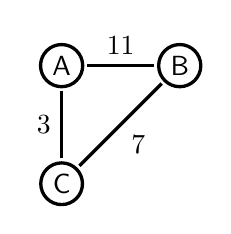
\begin{tikzpicture}[node distance=1.5cm]
                                \node[vertex]       (A) []                  {$\textsf{A}$};
                                \node[vertex]       (B) [right of=A]   {$\textsf{B}$};
                                \node[vertex]       (C) [below of=A]  {$\textsf{C}$};

                                \path [very thick]  	(A) edge [] node [above] {$11$} (B)
                                                                                (A) edge [] node [left] {$3$} (C)
                                                                                (B) edge [] node [below right] {$7$} (C);
        \end{tikzpicture}

        $p_{AB} = \frac{11}{14}, \; p_{BA} = \frac{11}{18}$.
    \end{center}
\end{halfboxr}

\begin{algo}{Disparity Filter}
    \textbf{Input:} A graph $G = (V(G),E(G))$. \\
    \textbf{Output:} A filtered graph $G' = (V(G'),E(G'))$.
    \tcblower
    \begin{enumerate}
            \item Select a threshold $\alpha \in [0,1]$.
            \item For every vertex, compute the relative significance score of every outgoing edge, i.e. the weight of the outgoing edge versus all of the vertex' outgoing edge's weights.
            \item Keep all edges which are significant for either of its endpoints, i.e. whose significance is larger than $\alpha$.
            \item Return the resulting subgraph.
    \end{enumerate}
\end{algo}

\end{document}
